\chapter{Related Work and Background} % Main chapter title

\label{chapter:relatework} 

In this chapter, we first introduce several game genres and games that we will refer to in the rest of this dissertation. We then review several theoretical foundations about player competence and engagement that we used. Next, we review existing endeavors in adaptive techniques that specifically target player competence and engagement in video games. Finally, we review churn prediction models, which quantify and predict churn as these are critical for our proposed recommendation systems.

\section{Game Background}

\subsection{Collectible Card Games (CCGs)}\label{sec:background_ccg}
 \textit{Collectible Card Games} (CCGs) is a class of games that is the basis of our proposed in-game item recommendation system for one-vs-one game settings, described in Chapter~\ref{chapter:qdeckrec}. CCGs have been popular since the 90s, evidenced by the large player base of these kinds of games. For instance, \textit{Magic: the Gathering} has more than 20 million players globally~\citep{guinnessmagic}, while an online free-to-play CCG \textit{Hearthstone} (Blizzard Inc.) reached a record of 40 million registered accounts in 2016~\citep{hearthstonepopular}. Since our experiments in Chapter~\ref{chapter:qdeckrec} is based on a simulator of Hearthstone, the rules we describe below are mostly based on Hearthstone; meanwhile, we note that many of them are shared by other CCGs.

A CCG typically has hundreds to thousands of different cards, each of which supports specific in-game rules and effects. When playing CCGs, before each match, every player is asked to build a \textit{deck} comprising of a subset of available cards. While in game, each player takes turns to draw cards from their respective deck and place them on the game board to combat (e.g., attack, counter-attack, cast spell, etc.) against their opponent cards. By default, a player only draws one card from their deck in each turn; however, certain cards' in-game effects allow them to draw more than one card. Cards can be mainly categorized as \textit{spells} and \textit{minions}. Spells are played, creating an effect on the battlefield, and then are discarded. Minions, on the other hand, stay in play, can be used to attack the opponent or other minions and endow extra abilities to the player such as drawing more cards from their decks. 

In a match, each player is initialized with certain health points. A match terminates by certain criteria, for example, whenever a player's health is destroyed. Each player is given a certain amount of mana in each turn. A player can play a card based on its associated rules, e.g., a card can be played when another card is present in hands and the player has sufficient mana to consume for playing this card. A player's turn ends when he or she has no actionable cards in hands or on the board, or voluntarily relinquishes the turn. A typical game flow of one-vs-one CCGs is shown in Algorithm~\ref{alg:ccg_1on1}. CCGs are match-based games because any actions in previous matches do not affect upcoming matches. At the beginning of each new match, all players' status get refreshed, such as health, their decks, and cards in hands and on the board.


%Algorithm~1 shows the typical game flow of the CCG. 
\begin{algorithm}
    \SetKwInOut{Input}{Input}
    \SetKwInOut{Output}{Output}
    \Input{$Player 1$, $Player 2$ with their customized decks}
    \BlankLine
    
    \While{game not end} {
    \BlankLine
	$curPlayer \leftarrow \text{alternate between } Player1 \text{ and } Player 2$ 
    
    \BlankLine
	$curPlayer$ draws cards from his or her own deck  
 
  	\BlankLine
    $curPlayer$ uses the cards in hands and in play to interact with the game
   		
  	\BlankLine 	
    }
    \caption{Game flow of one-vs-one CCGs}
    \label{alg:ccg_1on1}
\end{algorithm}

In general, there is no single deck which can universally win against all other decks. CCGs often design cards with sophisticated synergistic and oppositional relationships. For example, in Hearthstone, there are two distinguished types of decks that counter each other in different phases of a match. An \textit{Aggro} deck is considered as an aggressive archetype built with cards capable of dealing damage to the opponents as quickly as possible. In contrast, a \textit{control} deck is the opposite archetype with cards which can survive long enough to triumph in the late game through powerful but expensive cards or complex combos.

Based on the rules described, a player's in-game strategies and strength largely depends on what cards constitute the deck. Therefore, deck building is a crucial step prior to a match starts, with the goal to build winning-effective decks that suit the player's own play style and counter hypothetical opponents. There exist many online forums and websites for players to discuss, analyze and test deck building strategies (e.g.,~\cite{hearthpwn,icyveins}). However, deck building has a large and complex solution space and thus poses great challenges to players. For example, the number of all possible decks in our experiment setting (Section~\ref{sec:qdeckrec_exp}), which results from selecting 15 out of 312 cards, is $1.4 \times 10^{25}$. 

% The goal of deck building (or deck recommendation) is to identify a winning-effective set of cards which suits the player's own play style and effectively counters a target opponent.

The opponent's deck is invisible to the player prior or during the match. However we assume when a deck recommendation system recommends a deck to a player, it can access information of both players, including the player and the opponent's play styles, the opponent's deck built already. This assumption will be used in Chapter~\ref{chapter:qdeckrec}, where we propose a deck recommendation system to search for winning-effective decks against specific opponents. 


\subsection{Multiplayer Oline Battle Arena (MOBA)}\label{sec:background_moba}
Next, we introduce Multiplayer Online Battle Arena (MOBA) games since in Chapter~\ref{chapter:draftart} we will use MOBA games as a test bed for studying winning-effective hero recommendation in a team-vs-team setting.

% MOBA games have also attracted a variety of research thanks to their complexity and design richness as well as the publicly accessible datasets. Some research problems of interest include team formation analysis~\cite{pobie1,pobie2,neidhardt2015team,kim2016proficiency}, skill analysis~\cite{zhengxing2016player,Drachen:skill}, and hero pick recommendation systems~\cite{summerville2017reco,hanke2017reco}. A recent trend also attempts to build AI bots that can play at a professional human level~\cite{openaidota}. 

MOBA is one of the most popular contemporary E-sports games. Games such as \textit{League of Legends} (Riot Games) and \textit{DOTA 2} (Valve Corporation) have attracted millions of players to play and watch~\citep{lol_fanbase,lol_27million}. In a classic match within such games, two teams, each composed of five players, combat in a virtual game map (Figure~\ref{fig:moba_map}). The goal is to beat the opposite team by destroying their base. Each player controls an in-game character, known as \textit{heroes}~\footnote{We follow the terminology of DOTA 2.}, to co-operate with other teammates in attacking opponents' heroes, armies, defensive structures, and ultimately base, while defending their own in-game properties. We will keep referring to in-game characters in MOBA games as heroes, as this term is widely accepted by the player community. 

MOBA games are match-based games~\citep{guo2012analysis} as our definition in Section~\ref{chap1:motiv}, because they are played match by match: a new match starts with random 10 online players and ends whenever a team destroys the opponent's base. Records  within one match do not affect a new match, e.g., every player in a new match starts with level one of his or her character, the same amount of golds, and an empty item inventory.


\begin{figure}
\centering
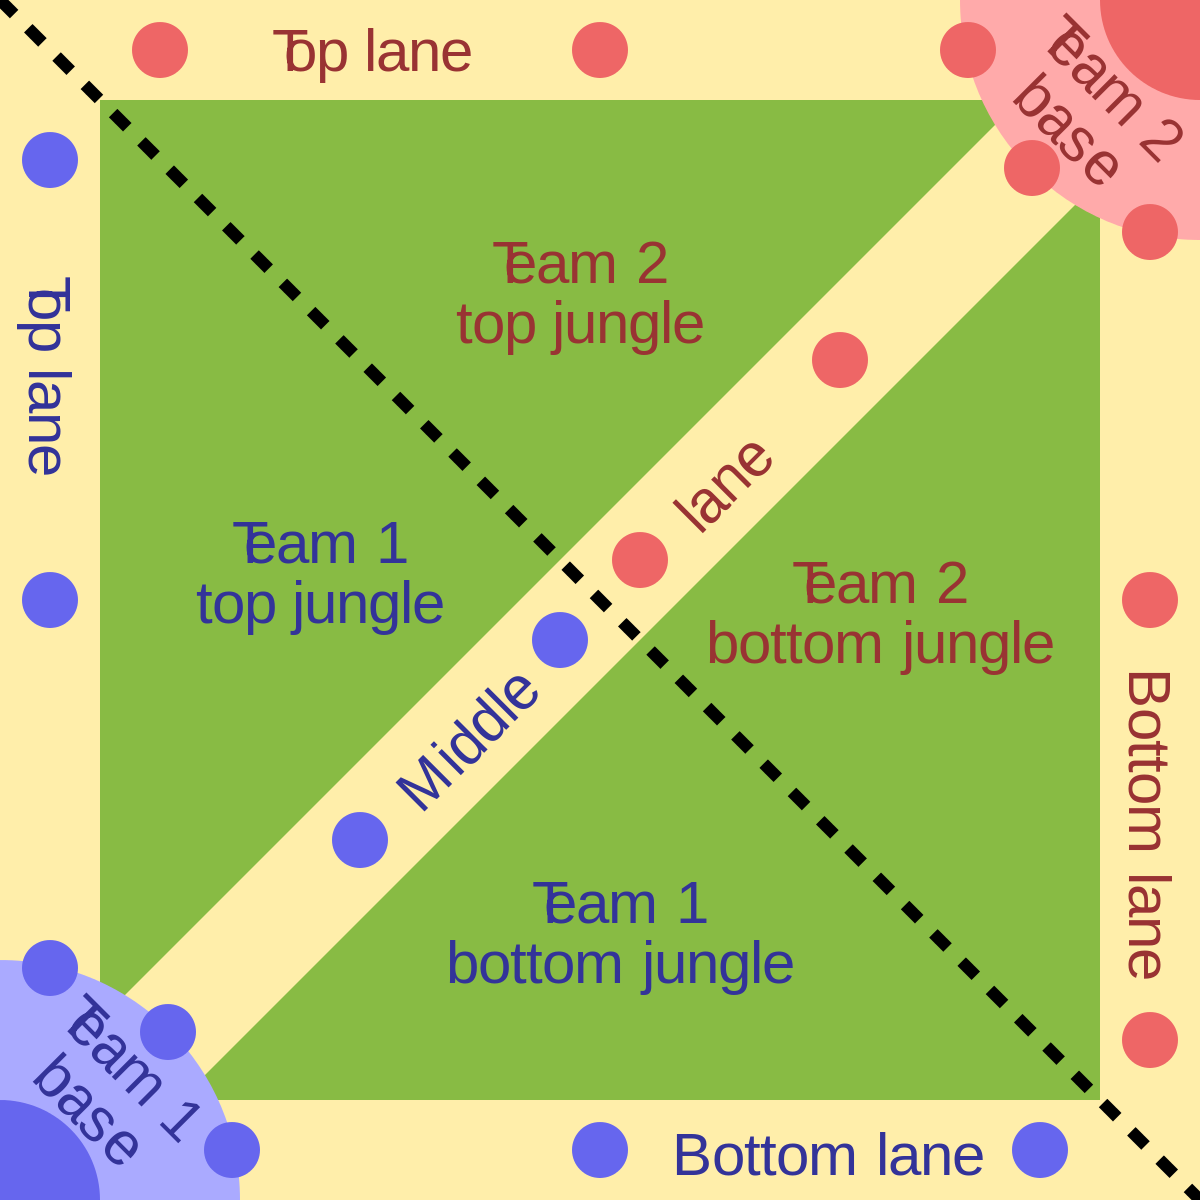
\includegraphics[width=0.6\textwidth]{Figures/map_of_dota.png}
\caption{The game map of DOTA 2. The bases of the two teams are on the ends of the diagonal. Player-controlled characters can move through lanes (Top, Bottom, and Middle) as well as partial areas of jungles. Most MOBA games have similar game maps like this one. Figure downloaded from the Internet: \url{https://bit.ly/2LbD3dv}}
\label{fig:moba_map}
\end{figure}

\begin{figure}
\centering
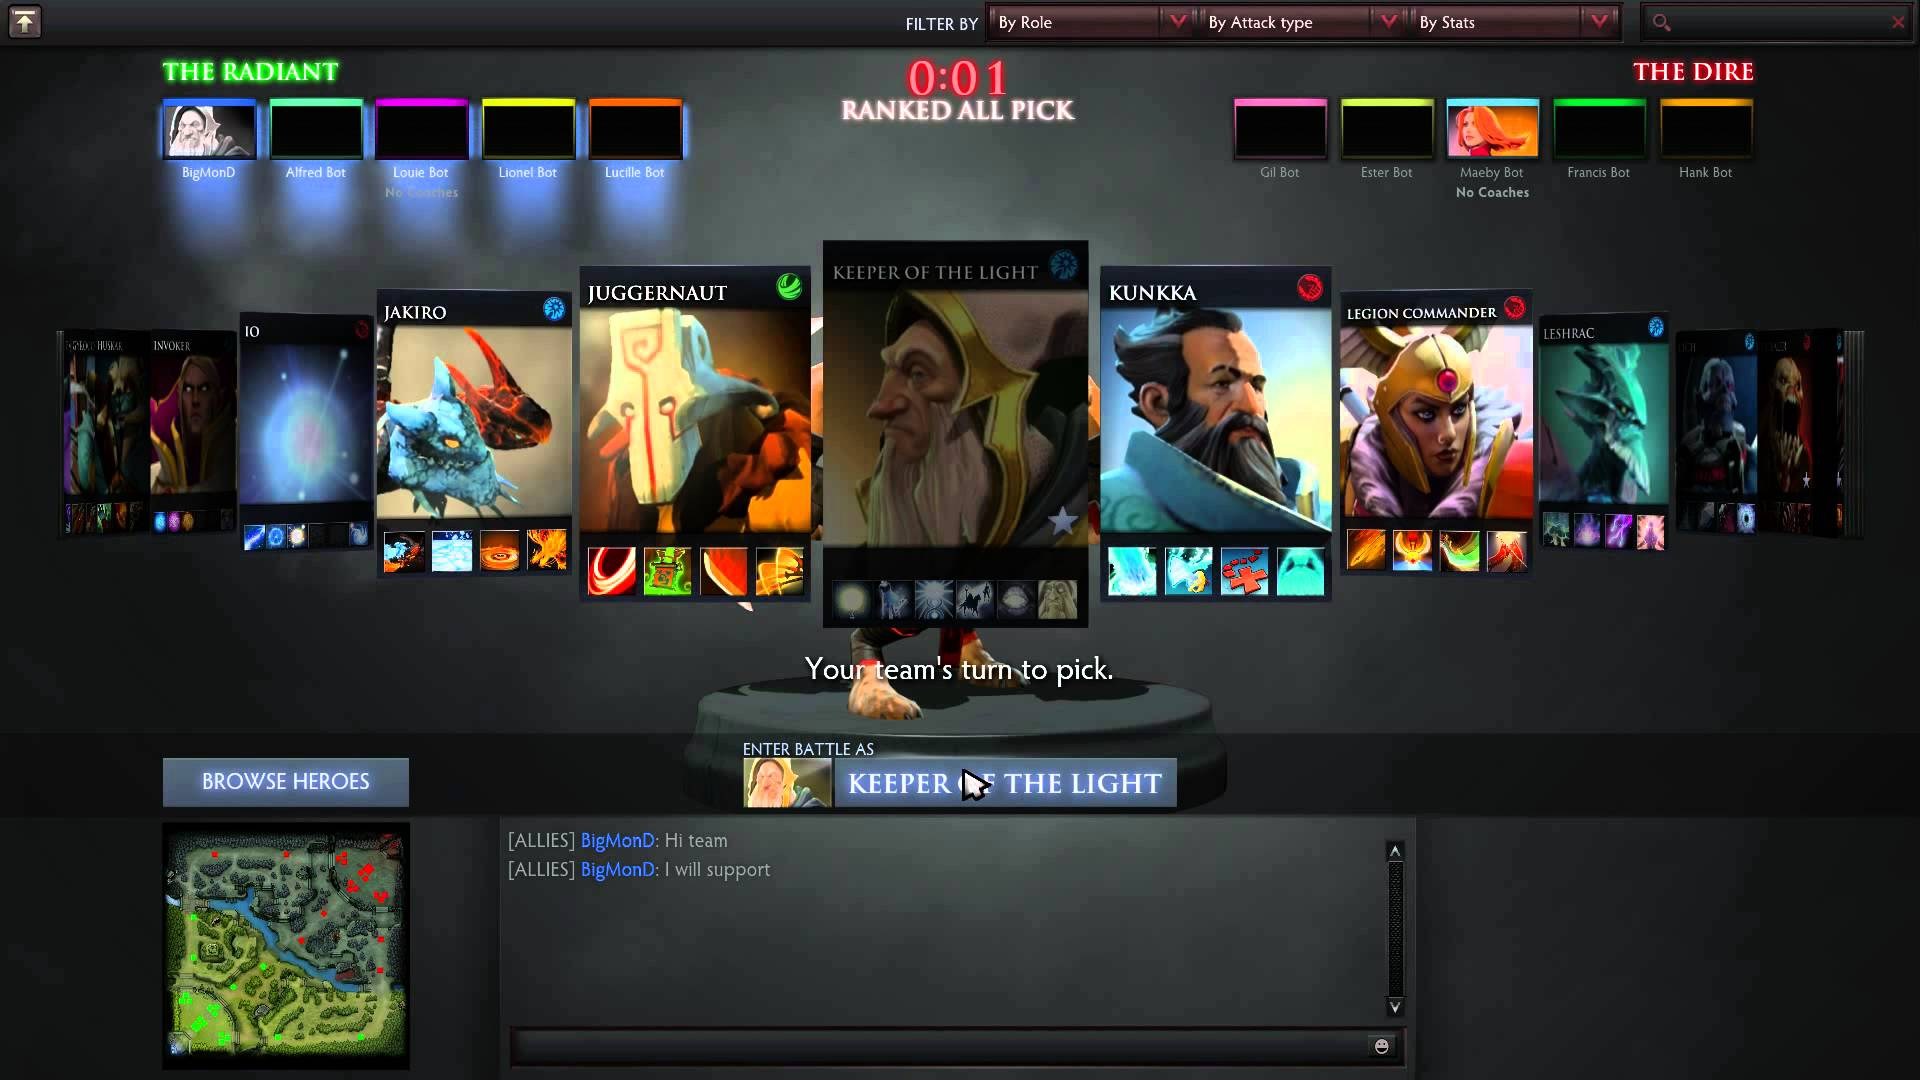
\includegraphics[width=1\textwidth]{Figures/ranked_all_pick.jpg}
\caption{Drafting interface in DOTA 2. Figure downloaded from the Internet: \url{https://bit.ly/2uBY8ni}}
\label{fig:ranked_all_pick_interface}
\end{figure}

Heroes are often designed with a variety of physical attributes and skills, e.g. dealing long-distance damage, healing teammates, or spearheading with strong shields, which together add to a team's overall power. Moreover, there exists sophisticated synergistic and oppositional relationships between heroes. For example, in DOTA 2, hero \textit{Clockwerk} has high synergy with \textit{Naix}, because \textit{Clockwerk} can transport \textit{Naix} to target enemies directly, making up for \textit{Naix}'s limited mobility in fighting. In another example, hero \textit{Anti-Mage}'s mana burn skill reduces an opponent's mana resource, making him a natural opposition to \textit{Medusa}, the durability of whom is completely reliant on how much mana she has. Previous research has also highlighted that interactions between heroes greatly influence match outcomes~\citep{pobie1,Semenov2016,kim2016proficiency}, as well as many online discussions about hero pick strategies \footnote{\url{http://www.weskimo.com/a-guide-to-drafting.html}}\textsuperscript{,}\footnote{\url{https://www.reddit.com/r/learndota2/comments/3f9szo/how_to_counter_pick_heroes/}}. 
 
 
The selection of heroes, also known as \textit{pick} or \textit{draft}, takes place before each match starts and alternates between two teams until each player has selected one hero. We refer to the 10 heroes in a completed draft as a \textit{hero line-up}. In a popular match mode named \textit{Ranked All Pick}, the alternating order of drafting is ``1-2-2-2-2-1'', meaning that the first team picks one hero, followed by the second team picking two heroes, then the first team picking two heroes, and so on. The process ends with the second team picking their last hero. During a draft, heroes already selected are visible to both teams. Heroes can only be selected from a fixed pool and no duplication is allowed in the same match. Moreover, a time limit (usually a few dozens of seconds) is imposed for each hero pick. Figure~\ref{fig:ranked_all_pick_interface} shows the interface for drafting in DOTA 2, where in the central area, a gallery of available heroes is presented for selection. In games like DOTA 2, there are possibly more than 100 heroes that can be picked by a player at the time of drafting. As estimated by~\textcite{hanke2017reco}, the number of possible hero line-ups in DOTA 2 is approximately $1.56 \times 10^{16}$. There are more sophisticated drafting mechanics and rules deployed and interleaved with hero picks in other match modes, such as \textit{banning} (i.e., certain heroes can be prohibited from selection by either team). To make illustration easier and simpler, we assume our system will be deployed under the Ranked All Pick mode (described above), unless otherwise mentioned in Section~\ref{sec:draftart_extension}.

Due to the complex synergistic and oppositional relationships among heroes and the large number of follow-up pick possibilities by other players, as we described above, the hero drafting phase becomes a critical component contributing to match outcomes. Selecting a winning-effective hero is a challenging task to human players especially inexperienced players ~\citep{johnson2015all}. Failing to pick heroes that fit teammates' currently selected heroes and counter opponent heroes may lower players' confidence and give rise to churn issues ~\citep{shores2014identification}, as well as behavioral issues, such as  flaming (i.e., aggressive, hostile, and profanity-laced blame of each other) ~\citep{kou2013regulating}, and cyberbullying ~\citep{kwak2015exploring}. All such issues negatively impact the experience of not only one player, but potentially the whole player community. Therefore, developing better systems that can minimize that issues would be important for such applications. 


\section{Theories of Player Engagement and Competence}\label{sec:related_theory_eng}

The primary motivation of this dissertation is to improve player engagement. A straightforward way to define player engagement is the "continued desire" to play the game repeatedly during the same session or over a longer period of time~\citep{schoenau2011player}. Player engagement is a complex construct that has been  studied extensively in many theoretical frameworks and linked to numerous aspects, such as emotions~\citep{sweetser2005gameflow,flow1990psychology,chen2007flow,cowley2008toward}, motivations~\citep{przybylski2010motivational,ryan2006motivational,yee2006demographics,yee2006motivations,sherry2006video}, presence~\citep{lombard1997heart,tamborini2006role}, immersion~\citep{mcmahan2003immersion,brown2004grounded,jennett2008measuring,ermi2005fundamental}, pleasure~\citep{costello2009tool}, enjoyment~\citep{ravaja2007fun,klimmt2003dimensions,mekler2014systematic}, fun~\citep{koster2013theory} and playability~\citep{federoff2003improving,federoff2002heuristics,desurvire2004using,nacke2009playability}.

One construct of player engagement which has been extensively studied is in-game challenge and competence. Within this construct player competence is defined by enjoyment of victory, accomplishment or dominance over other players while being appropriately challenged~\citep{ryan2006motivational,przybylski2010motivational,yee2006motivations,wu2010falling,sherry2006video,lazzaro2004we,schoenau2011player}. The theories introduced below will provide substantial support that providing proper competence to players will lead to better player engagement. which constitute the theoretical foundation for our work in recommending winning-effective in-game elements.

Self-Determination Theory (SDT)~\citep{ryan2000self}, a widely researched framework for the study of human motivation, has provided support for the importance of competence and its relationship to player engagement. Specifically, SDT defines three basic psychological needs for human motivation: \textit{autonomy} (the sense of volition or willingness when doing a task)~\citep{deci2000and,deci1964empirical}, \textit{competence} (the need for challenge and the feeling of being capable and effective)~\citep{white1959motivation,deci1985intrinsic}, and \textit{relatedness} (the feel of being connected with others)~\citep{ryan2001happiness,la2000within}. When the psychological needs are satisfied, people develop positive attitude and act effectively and hence experience well-being; however, if they are thwarted, people will more likely conduct negative behavior, such as prejudice and aggression. \textcite{ryan2006motivational} and \textcite{przybylski2010motivational} extended SDT and applied it to video games. They found that the three pillars of intrinsic needs (autonomy, competence, and relatedness) could be used to explain why people are engaged playing games. 

Flow~\citep{flow1990psychology}, as introduced in Chapter~\ref{chapter:intro}, is another theory highlighting that competence is an important building block of player engagement because players look for in-game challenge that commensurate with their skills. Flow  refers to the optimal mental state of engagement when a person is fully immersed and focused in their activities that he/she loses track of time~\citep{flow1990psychology}. The theory identified eight major components which lead to the Flow state, namely (1) a challenging activity requiring skill, (2) a merging of action, (3) clear goals, (4) immediate, direct feedback, (5) freedom to concentrate on the task, (6) a sense of control, (7) a loss of self-consciousness, and (8) an altered sense of time ~\citep{flow1990psychology}.   \textcite{sweetser2005gameflow} adapted the Flow theory to video games and attempted to map elements specific to video games to the eight major components of Flow, from which game design rules required for building engaging games are extracted. According to Sweetsser and Wyeth's mapping, the manifestation of the first component of Flow, ``a challenging activity requiring skill'' in video games is defined as ``challenges in games must match the players’ skill levels''~\citep{sweetser2005gameflow}.

Other theoretical works examining motivations underlying video game playing also discussed competition and challenge as important factors. The principle component analysis run by~\textcite{yee2006motivations} revealed three overarching motivation components: Achievement, Social, and Immersion. In this framework, Achievement includes competition referring to the desire to challenge and compete with others. \textcite{wu2010falling} verified Yee's three motivation components in the perspective of Uses and Gratification (U\&G) theory~\citep{palmgreen1985uses}, which posits that users actively seek out specific media that gratifies their specific needs. \textcite{wu2010falling} found that players' continued motivation is significantly impacted by the perception of gratification (i.e., Achievement, Social, and Immersion). \textcite{sherry2006video} identified 6 different gratifications of video game use, including challenge and competition along with social interaction, diversion, fantasy, and arousal. \textcite{lazzaro2004we} proposed four keys to release player emotions during play: Hard Fun, Easy Fun, Altered States, and the People Factor; Hard Fun refers to game challenges which frequently elicit emotions and experiences such as frustration and Fiero. Additionally, \textcite{schoenau2011player} explained player engagement as a process whereby players could feel positive affect through accomplishment (achievement, progression, and completion) and in turn be motivated to continue playing.  

 

% redefined it as a state of optimal match between a players' skills and the challenges presented by the game. 



\section{Data-Driven Models for Player Engagement}\label{sec:rw_data_player_engage}

Player engagement has also been investigated using data-driven approaches, where engagement is mostly measured quantitatively and behaviorally, such as purchases in the game~\citep{xie2015predicting,sifa2015predicting}, the number of matches played within a time window~\citep{xue2017dynamic,weber2011modeling}, or churn risk~\citep{hadiji2014predicting,harrison2012players}. Churn risk here is defined as the proportion of total players who stopped playing after a specific period of time. These metrics are proposed because they can be easily calculated from collected player data and reflect specific aspects of player engagement practitioners want to examine.

% Player engagement originally derives from user engagement prediction, which has been applied within various disciplines for decades, such as telecommunications \cite{ferreira2004data}, online advertisements \cite{yoon2010prediction} and insurance \cite{morik2004analysing}. 

% With the increasing popularity and collection of player data and adoption of data analysis models, several studies started to emerge on player engagement modeling and prediction. In these studies, player engagement is defined using several metrics, 

%  
We note some representative data-driven models for player engagement. They share a similar pattern that player engagement modeling is achieved through machine learning models trained to map from player states to engagement metrics.  \textcite{weber2011modeling} built  regression models to predict the number of games played by a player in a sport simulation game with features describing their game mode preferences, in-game performance and action choices.  \textcite{hadiji2014predicting} established a foundation to defining churn prediction in free-to-play (F2P) games. They proposed definitions for various churn behaviors and universal behavioral features, i.e., features \textit{not} game specific but shared across different F2P games such as session time and intersession itme. They then compared different machine learning models (decision trees, naive bayes, etc) across five commercial F2P games, they found that using decision trees could lead to high prediction accuracy.   \textcite{bertens2017games} proposed a scalable algorithm using conditional inference survival ensembles~\citep{hothorn2006unbiased} to predict both the level and accumulated time when a player leaves the game based on features.  The features they pick can easily be
generalized to other games and capture the temporal dynamics
of player behaviors, such as days since last purchase and days since last level up. The advantages of their model are the robustness to different data distribution and the ability to make a large volume of churn predictions in real-time due to being able to parallelized.

It should be noted that these prediction models, once trained, can be further interpreted to inform design issues or easily integrated into other systems. Based on their trained regression models, \textcite{weber2011using} further developed a technique to itemize the important features that can affect engagement prediction, drawing design recommendations that certain in-game controls should be simplified and more clearly presented. 
\textcite{runge2014churn} trained a churn prediction model for a casual social game and showed that such a model can be leveraged to decide the timing for delivering promotion campaigns that could increase the effectiveness of promotions. Churn prediction will also serve as an important building component in our opponent recommendation system proposed in Section~\ref{chapter:eomm}. 

\section{Techniques towards Improving Player Engagement}

Here we introduce three kinds of techniques related to our dissertation: Dynamic Difficulty Adjustment (DDA)~\citep{hunicke2005case}, Procedural Content Generation (PCG)~\citep{yannakakis2011experience,togelius2011search} and Recommendation System~\citep{medler2011using}. We will first overview the three kinds of techniques and their relationships, and then introduce each of them in more details.

DDA~\citep{hunicke2005case} aims to keep players' perceived competence in the optimal zone to accomplish a state of flow~\citep{flow1990psychology,sweetser2005gameflow,chen2007flow} through manipulating game difficulty adaptively. Such systems are related to our work  because recommendations of winning-effective in-game elements, which we study in \hyperref[rq1]{\textbf{R.S.Q.~1}} may also cause difficulty and player competence may thus change, if players adopt the recommendations. Therefore, in our opinion, techniques we will investigate to answer \hyperref[rq1]{\textbf{R.S.Q.~1}} are also within the area of DDA. PCG~\citep{yannakakis2011experience,togelius2011search} refers to methods that automatically (or algorithmically) generate adaptive in-game content. Recommendation systems are used as information filtering tools to  present specific in-game elements from a pool of candidates~\citep{medler2011using}.  It should be noted that DDA  involve various techniques borrowed from both PCG and recommendation areas, and PCG and recommendation systems can be used for various goals including DDA. 

% These systems are directly related to the work described here and thus we will discuss them in more detail.

% Inspired by the theoretical works on player competence and  engagement introduced above, two forms of techniques have been mainly used, based on our literature review, for manipulating player competence: dynamic difficulty adjustment (DDA) and recommendation systems.


\subsection{Dynamic Difficulty Adjustment}\label{sec:dda}

A straightforward way to manipulate game difficulty is \textit{rubber banding}, which means the difficulty of the game rises or falls if the player plays well or poorly. A famous example is from \textit{Mario Kart} series (Nintendo Co., Ltd), in which players who lag behind are more likely to get power-ups to speed them up and thus catch up to front runners. 

Rather than having a monotonous approach to difficulty adjustment for all players, more advanced works leverage player modeling~\citep{yannakakis2013player} as a tool to identify more granular players' preferences and deliver more personalized difficulty adaptation~\citep{missura2009player,zook2012temporal}. They are inspired by the fact that different types of players desire for different scales of difficulty and player skills may vary along time. For example, dealing with the first fact, \cite{missura2009player} proposed to categorize a player into one of a few player clusters based on a short play trace of the player then adjust difficulty suitable for that particular player cluster. Dealing with the second fact, \textcite{zook2012temporal} proposed to use tensor factorization techniques~\citep{kolda2009tensor} to fit player performance data collected historically, which can then be used to forecast player skill mastery in the future.

Another notable kind of advanced models is to formulate difficulty adjustment in a more rigorous probabilistic framework, which enables in-depth analysis of system performance. For example,  \textcite{missura2011predicting} formulated adjusting difficulty as an online learning problem~\citep{auer1995gambling} in which the ranking of finite game difficulty settings is estimated through a trial-and-error fashion with the goal to choose the ``just right'' difficulty setting as often as possible. The probabilistic framework guides the system to select the proper difficulty setting that is most likely to match the player’s skill (which could even vary temporally) while providing a theoretical bound on the number of mistakes the system would make. 

The ways to deliver difficulty adjustment can be as simple as tuning pre-defined parameters which govern environmental changes (e.g., adjusting supply and demand when players are close to death in~\cite{hunicke2005case}) or player attributes (e.g., awarding shield and health points to low-performing players in~\cite{baldwin2014effect}), or can be as sophisticated as AI-controlled agents that could adapt to players' gameplay. The goal of AI-controlled agents for DDA purpose is to select and perform behaviors (actions) leading to small outcome gaps. Back in 2004, \textcite{spronck2004difficulty} equipped dynamic scripting~\citep{spronck2004online}, an online learning based behavioral script technique, for agents to adapt their behaviors to achieve roughly equal win/loss ratio against opponents. In dynamic scripting, an agent's behavior is sampled from a rulebase system, where each rule (behavior) is associated with a sampling weight that determines how often this rule should be sampled. Rule weights are learned in a training phase based on \textcite{spronck2004difficulty}'s proposed techniques in order to scale the intelligence level of the agent to the level of the opponent. Andrade and his colleagues applied Q-Learning~\citep{watkins1992q}, one family of Reinforcement Learning algorithms~\citep{sutton1998reinforcement}, to estimate action values in an offline training phase. Then, in the play time after training, every $\tau$ time steps an agent would take the action with its value ranked in 50 percentile of all valid actions, where $\tau$ is a dynamically changing parameter reflecting how rapidly the difficulty needs to be adapted to commensurate with player skill~\citep{andrade2006dynamic,andrade2005challenge,andrade2005extending}. To overcome the fact that the 50-percentile ranked action might not always be the best action to balance the game and to reduce the manual effort to tune the parameter $\tau$, \citep{demediuk2017monte} equipped AI-controlled agents with Monte Carlo Tree Search~\citep{browne2012survey} in another fighting game for fully automatically determining actions that are promising to lead to the minimal outcome gap. 

Several works have conducted experiments and shown that player engagement-related metrics indeed improve due to the use of the proposed methods. In the work by~\textcite{hunicke2005case}, the author adjusted supply and demand in a game and finds that expert players reported slightly elevated levels of enjoyment (although novice players did not). In the work by~\textcite{van2009incongruity}, players reported to have decreased pleasure and increased frustration when playing harder games compared to balanced games. ~\textcite{xue2017dynamic} deployed a difficulty adjustment system to a commercial matching-three game (a game like \textit{Candy Crush}). They discovered that difficulty adjustment could bring as much as $7 \sim 9 \%$ improvement in total numbers of rounds played and duration of gameplay. Using a crowdsourcing science game, \textcite{sarkar2017engagement} found that presenting 
tasks in skill-based difficulty ordering to players led to significantly more attempted and completed levels than random ordering. 

\subsection{Procedural Content Generation}\label{sec:pcg}

Procedural Content Generation (PCG) is the algorithmic generation of game content with limited or indirect user input~\citep{yannakakis2011experience,togelius2011search}. The goal of applying PCG is not only to eliminate some of the content development burden for developers, but to also adapt game content to satisfy players' dynamic needs. \textcite{togelius2011search} provides a comprehensive taxonomy of different PCG algorithms, such as online-vs-offline (whether game content is generated during the run time or development time of the game), random-seeds-vs-parameter-vectors (generation up to a single seed or a series of specifications), etc.

PCG has been used for various purposes, such as adjusting difficulty and player engagement, depending on what the underlying evaluation function is for assessing generated content. An example of applying PCG for difficulty adjustment is an early work from ~\textcite{jennings2010polymorph}, in which levels of a platformer game are automatically generated segment by segment, where the next segment was generated with the difficulty level appropriate for how the player performs in the current segment. This relies on a machine learning model (Multilayer Perceptron) which learns the mapping from level specifications to difficulty reported by players themselves. On another platform game, PCG is applied to optimize player engagement~\citep{shaker2012evolving}, with a player engagement prediction model used to guide the generation of levels. The player engagement prediction model, also a Multiplayer Perceptron model which is based on their former works~\citep{shaker2011feature}, is constructed to predict player's reported level of engagement using features of level characteristics and players' playing styles.

Although PCG and recommendation systems are both valid and potential ways to improve player engagement, we focus on the latter in this dissertation. As we introduced in Chapter~\ref{chapter:intro}, studying PCG would require access to some testbed games for modification of game content, which was not available to me during my research. Therefore, we primarily study recommendation systems which rely on collected data and simulators.

\subsection{Recommendation Systems}\label{sec:recsys}

% Rather than directly manipulating in-game elements like DDA, recommendation systems are used as information filtering tools to dedicatedly recommend to players specific in-game elements from a pool of candidates which are assumed to be generated already by the game~\cite{medler2011using}.


Recommendation systems have been studied for long in a variety of areas such as movies~\citep{amatriain2012netflix}, e-commerce~\citep{linden2003amazon} and news~\citep{das2007google}. The primary goal of these recommendation systems is to serve as information filtering tools to ease information overload, retrieve the most relevant information, and provide personalized services~\citep{isinkaye2015recommendation,bobadilla2013recommender,resnick1997recommender,adomavicius2005toward}; without such systems, users would be confronted with millions of items with no guidance on how to search such a large space. These recommendation systems predict users' preferences on items accurately such that personalized item recommendations can be given based on the ranking of user preference predictions~\citep{liang2006personalized}. 

The video game industry has also used recommendation systems to introduce players to games that they are likely to enjoy~\citep{sifa2014archetypal,orland10,skocir2012mars,wu2017recommendation}. These recommendation systems, like their counterparts in other web-based services, alleviate information overload faced by users, as users are not able to go through all candidate games as this is usually a prohibitively large list. 

Video games as a form of interactive entertainment allow game developers to apply recommendation systems not only for recommending next games to play, but also to recommend in-game elements for a particular game. In this dissertation, we focus on recommendation systems for in-game elements within match-based video games which have  features different from traditional recommendation systems introduced in the previous paragraph. First, our goal is focused on predicting in-game elements' influences on winning-effectiveness and engagement, which may be manifested by metrics like winning probabilities, rather than players' preferences. Second, in-game element recommendations to one player may affect other players' experience. Therefore, in-game element recommendations have to consider other players. This is different from traditional recommendation systems where recommended items to one user are relatively independent from other users' experience.

% Although in-game element recommendation systems have been utilized for a variety of purposes~\citep{kolen2018horizontal,wu2017recommendation}, 

In-game element recommendation systems sharing the same scope as this dissertation have only sporadic appearances in literature (i.e., in-game element recommendations in the pre-match stage in match-based games for influencing player competence and engagement). Our suspicion for the lack of research in this area is that access to data from large-scale commercial games, which have sufficiently sophisticated in-game elements to apply recommendation system techniques to, is hard to come by. The difficulty may drive academic research to focus only on a few publicly accessible datasets or games with a smaller scale of which researchers can have full access and control. Nevertheless, we survey existing works as follows, with each subsection corresponding to recommendation systems that cope with a specific type of in-game element we will investigate in Chapter~\ref{chapter:qdeckrec},~\ref{chapter:draftart}, and~\ref{chapter:eomm}, respectively.

% (e.g., starting gifts in Dark Soul and starting weapons in Bloodborne)

\subsubsection{Starting Item Recommendation}\label{sec:rw_startitem}
Starting items are commonly seen in-game elements in a variety of genres of games, such as Action Role-Playing Game (Action-RPG) and Multi-Player Online Arena (MOBA), where starting items aid in-game characters heal, scout, defend, and attack when characters are weak in their initial stages. In Collectible Card Games (CCGs) starting items are a set of cards, called a \textit{deck} (See CCG background in  Section~\ref{sec:background_ccg}). Some games have incorporated starting item recommendation features; for instance, when making purchases of starting items in League of Legends, players can browse the full list of all items or a short list of recommended items for easier choices~\citep{lol_recomitem}. However, to the best of our knowledge, the underlying recommendation techniques in commercial games are largely undisclosed, probably due to proprietary reasons.

Despite the prevalence of starting items in video games, to the best of our knowledge, we have only seen little academic research in starting item recommendation. Specifically in the problem of deck recommendation for one-vs-one CCGs, which we discuss in Chapter~\ref{chapter:qdeckrec}, we have only seen search-based solutions using either heuristic search or metaheuristic search~\citep{birattari2009tuning}.

% However, neither of the search methods is efficient to deploy for large-scale or real-time deck recommendation. 

Heuristic search methods suggest which cards to include in a deck based on domain heuristics such as popularity and in-game resource curve~\citep{frankkarsten,willfancher,stiegler2016hearthstone}. However, they require in-depth human knowledge and lack flexibility to adapt to different play styles and opponents. Metaheuristic searches rely on high-level, problem-independent, approximate search strategies for tackling optimization problems~\citep{birattari2009tuning}. Researchers have used one type of metaheuristic search called \textit{Genetic Algorithm} (GA)~\citep{holland1992adaptation} to evolve decks towards higher winning-effectiveness through repeated modifications and selections~\citep{garcia2016evolutionary,bjorke2017deckbuilding}. In GA~\citep{holland1992adaptation}, candidate solutions (called \textit{individuals}) evolve towards better feasible solutions iteratively with \textit{mutation} and \textit{crossover} operators. In each generation, the \textit{fitness value} of every candidate solution is evaluated. The fitness value is usually the value of the objective function in the optimization problem being solved; in the works of ~\textcite{garcia2016evolutionary} and \textcite{bjorke2017deckbuilding}, the fitness value is the average win rate of a candidate deck against a group of opponent decks while AI bots are used as a proxy for human play. The fit candidate solutions are stochastically selected and modified to form a new generation. Although not requiring human knowledge to guide searches, metaheuristic search algorithms incur a large computational cost for simulation-based evaluation on intermediate solutions, which renders them unsuitable for large-scale or real-time usage. In Section~\ref{sec:qdeckrec_existmethodanaly}, we will analyze in details why existing approaches are inefficient.

\subsubsection{Character Recommendation}\label{sec:rw_character}
The rich design of characters and recent worldwide popularity of MOBA games have allowed them to become the primary testbed for character recommendation research. Classic MOBA games, like League of Legends and DOTA 2, are usually played 5-vs-5; there are possibly more than 100 characters that can be picked by a player in the pre-match stage. Moreover, as per rules of certain match modes players are supposed to select characters in sequence; players need to consider synergistic and oppositional relationships among champions because a winning-effective character should not only fit to selected characters so far but also projected characters selections by the rest of players. 

To recommend winning-effective characters in the character selection phase, \textcite{hanke2017reco} proposed to mine association rules~\citep{agrawal1994fast} from historical character selection data and use them as the heuristic to recommend heroes. Here, association rules are character subsets that appear frequently together either in the winning team or in opposite teams. Any character contained in the discovered association rules together with characters picked already is suggested to be a good candidate to pick next. However, this method does not consider which characters \textit{will} be picked by other players in the rest of the drafting process, hence this is essentially a myopic, greedy-based approach.

% Previous works on hero pick recommendation can be categorized into two main approaches, based on (1) historical selection frequency, and (2) previous win rate.

Researchers have also proposed to recommend characters based on player selection tendency. \textcite{summerville2017reco} models character recommendation as a sequence prediction problem. They train a sequence prediction model for predicting the next character most likely to be selected based on historical character selection sequences. However, the predicted character is ``what is
likely to be picked, not what is necessarily best''~\citep{summerville2017reco}. Therefore, character recommendation based on such a method may not be an optimally winning character for team victory.

Although there are other works predicting match outcomes~\citep{Yang:identifying,Semenov2016,makarov2017predicting} and analyzing in-game traces~\citep{cavadenti2016did}, they do not focus on how to utilize these models for character recommendation in the context of sequential character selection.


\subsubsection{Matchmaking (Opponent Recommendation)}

% My\'{s}lak and Deja 
% Delalleau et al. 

In practice, the concept of opponent recommendation is often implemented as matchmaking services, which connect players to form matches. As such, players themselves become the subjects of recommendations.

% Jim{\'e}nez-Rodr{\i}guez et al.

A fair amount of matchmaking systems simply assume that skill balanced games are good for engagement \citep{graepel2006ranking,sweetser2005gameflow,flow1990psychology,chen2007flow} and hence resort to skill rating algorithms~\citep{glickman1999parameter,elo1978rating,herbrich:trueskill} to identify similarly skilled opponents. \textcite{myslak2014developing} suggests additional information about player preferences in in-game avatar roles can further improve fairness-based matchmaking systems. A few researchers have explored methods to improve player engagement through matchmaking. \textcite{Delalleau2012} proposed to train a neural network based architecture which predicts player enjoyment based on their historical statistics. They measured enjoyment by directly asking players for feedback after each match. However, their enjoyment-based matchmaking has not been verified in real games. Plus, whether players are willing to give feedback about enjoyment and how reliable their feedback would be are questionable. \textcite{jimenez2011matchmaking} proposed that matchmaking could be based on preferred roles by players. They argue that a fun match should have players act in  roles with perceivably joyful role distribution. However, it is still a conceptual, heuristic-based method without experiment showing that such matchmaking system indeed improves concrete engagement metrics. To our best knowledge, we have not seen any existing opponent recommendation method that formally treats the opponent recommendation task as an optimization problem to maximize player engagement. 







% Each CCG has a fundamental set of rules that describes the players' objectives, the categories of cards used in the game, and the basic rules by which the cards interact. The CCG that we will use is 1-vs-1 and turn-based. In a match of the CCG, two players take turn to make movements. Each player is initialized with certain health points. The victory objective is to destroy the opponent's health by playing the cards in possession. Each player is also initialized with certain mana points. Mana points get refresh in each turn and increase as the game proceeds. One card is drawn from the player's \textit{deck} to his hands at the beginning of his each turn. Deck is a collection of cards that the player selects from an available pool of cards before the match starts. After the draw, the player uses the cards he has drawn to his hands to interact with the game in order to gain an advantage over the opponent. Each card is assigned with a fixed mana cost. When a card is played out of his hands, it costs the designated amount of mana from the player. The player's turn ends when he has no available actions to perform or he voluntarily relinquishes his turn. 

% Each card is associated with effects, attributes and rules to play it. There are two types of cards, \textit{Minion} and \textit{Spell}. Minion cards, when cast from the player's hands, stay in the game helping the player attack and defend until the opponent takes actions to eliminate them. Spell cards will adjust the game environment as per their designated effects, for instance, one-time damage to opponent or his minions, or recover health to the player or his own minions, or summon new minions. 

% Deck is the initial equipment in CCGs. Because the size of total available cards (usually hundreds or thousands) is much larger than the size of deck (usually a few dozens), CCG players need to strategically customize their decks to take advantage of favorable card interactions, combinations and statistics. However, some inexperienced players have too limited knowledge to construct a competent deck to win a match. 

% Therefore, players need to draft heroes that can enhance the strengths and compensate for weaknesses of teammates' heroes (i.e., \textit{synergy}), while posing suppressing strengths over those in the opponent team (i.e., \textit{opposition}).

% The pursuit of victory and achievement is a common reason of player engagement~\cite{schoenau2011player,yee2006motivations,sherry2006video,wu2010falling,lazzaro2004we}. Victorious or progressive game outcomes can be seen as one kind of fulfillment of victory and achievement. Also, players look for the level of competitiveness commensurate with their skills. Central to the flow theory proposed by Cs\'{i}kszentimih\'{a}lyi~\cite{sweetser2005gameflow,flow1990psychology,chen2007flow} is the idea that there should be an optimal match between the skills an individual possesses and the challenges presented by an activity. Similarly, competence is one of the three pillars in Self-Determination theory~\cite{przybylski2010motivational,ryan2006motivational}, which refers to people's desire for challenge and feelings of mastery as their intrinsic motivation to engage in the game. Therefore, monotonous match outcomes are not desirable because they indicate consistent over-/under-challenging player experience. 

% , which 

% Many commercial games have also adopted dynamic difficulty adjustment, such as .

% This raises the importance to carefully maintain the winning rate for players, especially those inexperienced players who have difficulty of winning a match.

% It is important to note the relationship between our proposed pre-match personalized recommendation techniques and the existing studies on player engagement and match outcomes. The initial item recommendation aims to recommend the optimal initial items to maximize one's win rate, i.e., to influence match outcomes positively to the largest extent. Therefore, it is a direct method to affect match outcomes but needs additional cares if used to improve player engagement. The opponent recommendation uses the player engagement as a criteria to seek personalized opponents and adjust match outcomes. Therefore, it simultaneously affects match outcomes and player engagement.

% The tight relationship between game outcomes and player engagement raises the importance to carefully maintain the proper pace of game outcomes that players would experience. One way is to use recommendation system techniques~\cite{medler2011using} to dedicatedly present in-game elements to players such that their in-game decisions and behaviors could be influenced to eventually impact game outcomes.

% Empirical studies also indicate that game outcomes are correlated with player engagement, mostly coming from the topics of churn prediction and dynamic difficulty adjustment. On the one hand, data-driven models for predicting churn behaviors often rely on features derived from game outcomes. \cite{weber2011using} build a regression model for predicting the number of games played for each player in a football game, while observing the win ratio of certain game modes are influential in the prediction. Similar application of using game outcomes-derived features for churn prediction models can also be found in~\cite{harrison2012players,xie2015predicting,}. 

%, not necessarily a permanent churn. 
% We define churn risk as the proportion of total current players who will stop playing the game over a period of time. 
% Various recommendation techniques have been applied in both stages. For example, in the pre-match stage, opponents can be recommended to match the player's skill level in order to make games sufficiently challenging~\cite{sweetser2005gameflow,flow1990psychology,chen2007flow} and winning-effective characters, starting items. In the in-match stage, tactical and strategical hints suitable to players knowledge level~\cite{weber2009data,cunha2014rtsmate} can be recommended in order to help players with difficulty of winning the match and prevent disengagement from frustrating experience~\cite{schoenau2011player}.

% We will use two subsections to discuss the state-of-the-arts in initial item recommendation and opponent recommendation.


% \subsubsection{Deck Recommendation}~\label{deckrec_prev}
% Deck recommendation is a novel topic which have been studied by only a few works. The existing works can basically be divided into two directions. First, intuition-driven methods decide which cards to be included based on the popularity of cards from collected historical data~\cite{frankkarsten,willfancher}. The underlying intuition is that popularly used cards are very likely to be strong ones as a result people favor them. However, these methods do not guarantee the assembled deck of the most popular cards is competitive. Stiegler et al.~\cite{stiegler2016hearthstone} propose a utility system to search deck with more types of game-specific heuristics added besides card popularity, including mana curve, strategic parameters, cost effectiveness and card synergies. However, all intuition-driven methods are manually heavy and not easy to transfer to other games intelligently. Second, Garc{\'\i}a-S{\'a}nchez et al.~\cite{garcia2016evolutionary} proposed to use Evolutionary Algorithm~\cite{simon2013evolutionary} to iteratively modify decks and select ones with faithful fitness values imitating the process of natural evolution. The fitness value is the average win rate of the candidate deck pitting against a few common used decks while a default, greedy-based AI is used for both sides in every match. However, the limitation of their method is that a deck's strength may not be completely realized by just using the universal, greedy-based AI as used in the fitness value evaluation. Moreover, the evolution of candidate decks is currently totally random
% rather than following some logical sense similar to human players. For example, rather than randomly replacing a card with another card, they do not want to break good card combinations or replace a card with a similar but much weaker one. As a result, the fitness landscape in the current EA algorithm~\cite{garcia2016evolutionary} is quite agitated and the process to find an ideal deck requires a large computational cost. Furthermore, the EA-based deck recommendation is not reusable. Each time a deck is asked to recommend, the EA-based deck recommendation has to restart the whole process of evolution without any prior deck search experience transferred. Therefore, the EA-based algorithm is not a practical implementation if deck recommendation needs to be requested in a large scale. For example, game companies might want to implement a deck recommendation API to serve a large population of new players.


 



